A fairly scientific method was used to determine a reasonable value for the range parameter. The following steps were taken to compute a reasonable value for the range: 

\begin{enumerate}
    \item What if the coverage was a square? Assuming a system with $n$ balloons, what is the size of each square patch?
    \item What is the size of the larges square patch that one circle can cover?.
    \item Infer answer from 1 and 2.
\end{enumerate}

The notations in the calculations map with the model parameters as stated here:

\begin{align}
    x &= \text{WORLD\_SIZE}\notag \\ 
    r &= \text{RANGE}\notag \\
    n &= \text{NUMBER\_OF\_BALLOONS} \notag \\
    a &= \text{Distance from circle center to edge of inner square} \notag \\
    A &=\text{Area of inner square of a circle} \notag \\
\end{align}

The world is a grid with area 
\begin{align}
S=x^2 \notag
\end{align}

The number of balloons is $n$ so each one is responsible for covering an area of size $\frac{x^2}{n}$. The distance from the center of a circle to the edge of its inner square is

\begin{align} 
a^2 + a^2 &= r^2 \notag \\
a &= \sqrt{\frac{r^2}{2}} \notag
\end{align}

but that means that the are of the inner square is

\begin{align}
A &= \frac{r^2}{2}
\end{align}
The goal was to fill the area $S$ but that means
\begin{align}
A &= S\notag \\
\iff \frac{r^2}{2} &= \frac{x^2}{n}\notag \\
\iff r &= \sqrt{\frac{2}{n}}\cdot x \notag \\
\iff RANGE &= \sqrt{2} \cdot \frac{WORLD\_SIZE}{\sqrt{NUMBER\_OF\_BALLOONS}} \notag
\end{align}
\begin{figure}[H]
    \centering
    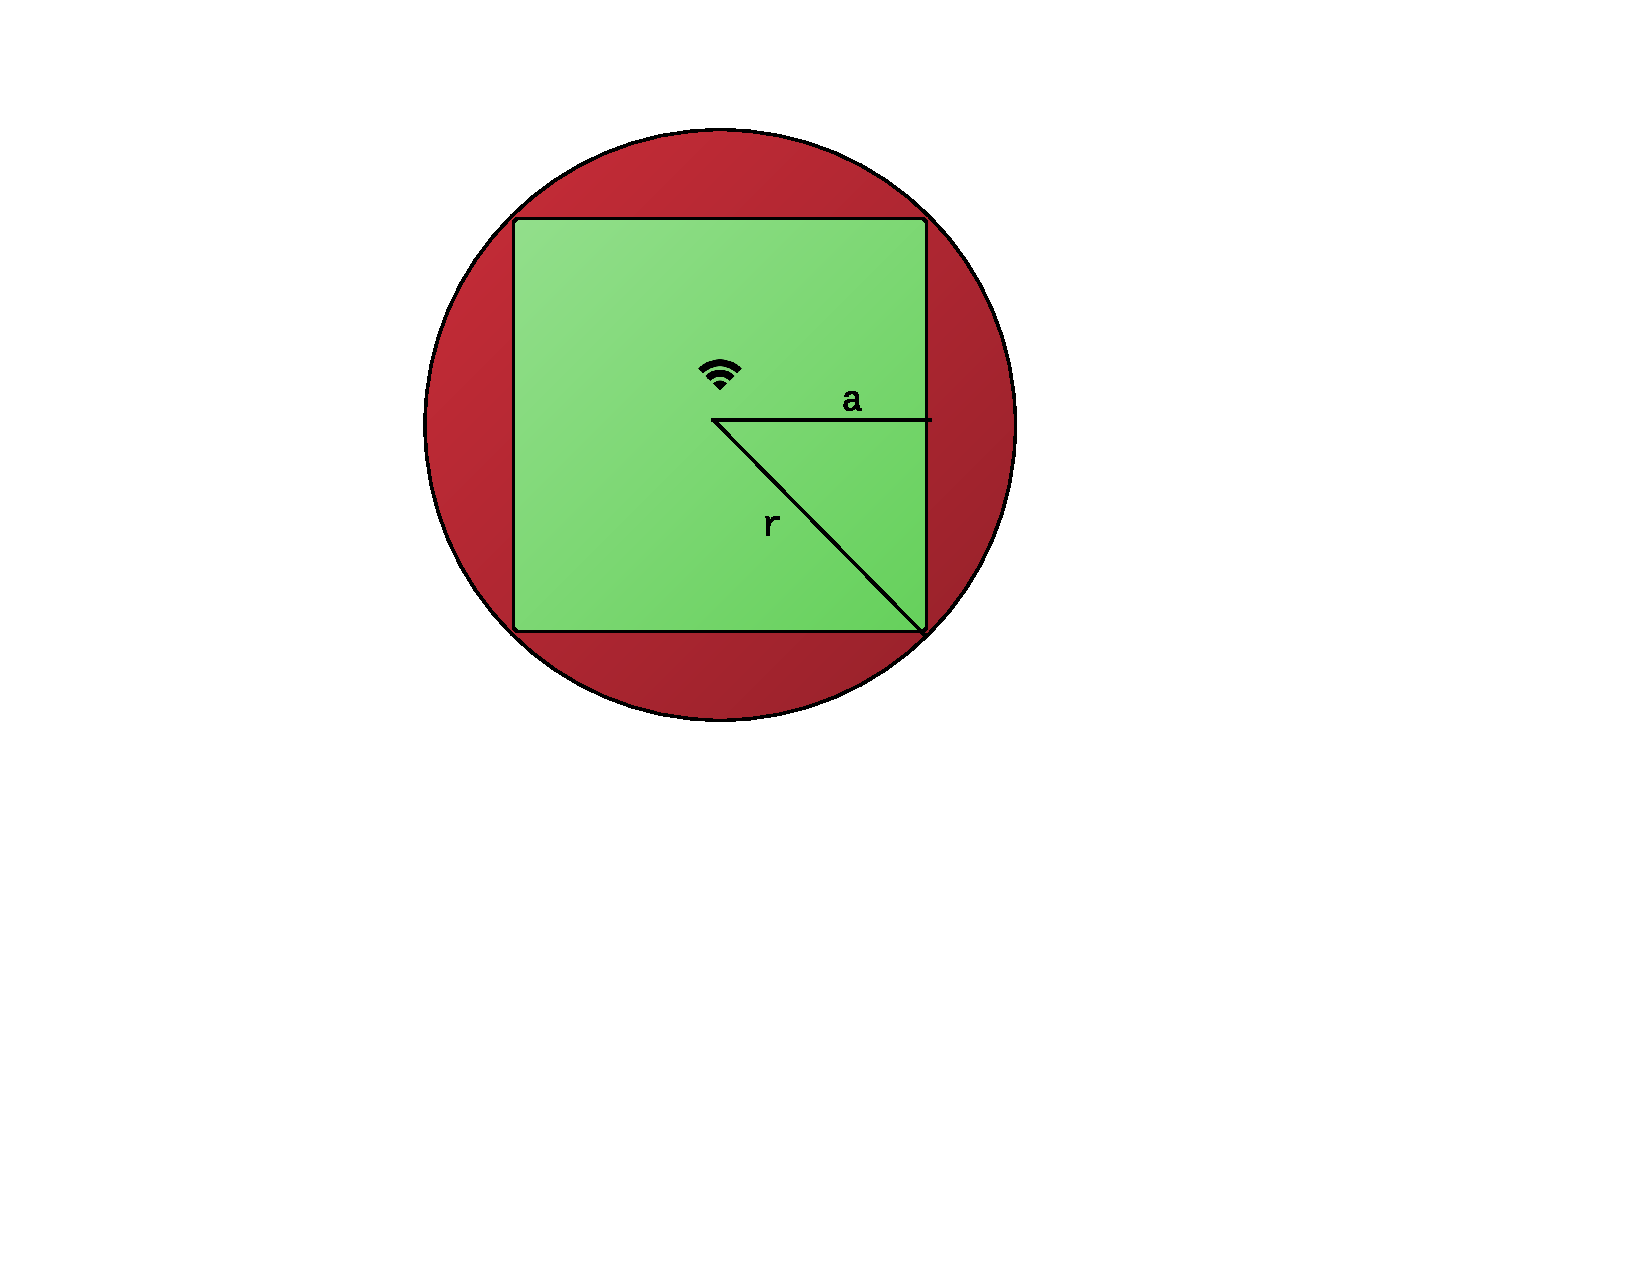
\includegraphics[scale = 0.5,trim=3cm 8cm 6cm 2cm, clip]{graphics/innersquare.pdf}
    \caption{Variables used for calculation of inner square}
    \label{fig:innersquare}
\end{figure}

Range is of course rounded to the next whole integer as the world is represented with an integer grid. But why programming this dependency between the model parameters range, world size and number of balloons? This model is an abstract version of the world and void of any units for length or size so controlling the ratio between the range versus the size of the grid is meaningless. This choice of range will clearly cover more than the actual area as displayed in figure \ref{fig:innersquare} but this is as good of a starting point as any. Modifying and exploring the effect of a smaller or larger range is of course possible and straight forward.